%%%%%%%%%%%%%%%%%%%%%%%%%%%%%%%%%%%%%%%%%
% Journal Article
% LaTeX Template
% Version 2.0 (February 7, 2023)
%
% This template originates from:
% https://www.LaTeXTemplates.com
%
% Author:
% Vel (vel@latextemplates.com)
%
% License:
% CC BY-NC-SA 4.0 (https://creativecommons.org/licenses/by-nc-sa/4.0/)
%
% NOTE: The bibliography needs to be compiled using the biber engine.
%
%%%%%%%%%%%%%%%%%%%%%%%%%%%%%%%%%%%%%%%%%

%----------------------------------------------------------------------------------------
%	PACKAGES AND OTHER DOCUMENT CONFIGURATIONS
%----------------------------------------------------------------------------------------

\documentclass[
	a4paper, % Paper size, use either a4paper or letterpaper
	10pt, % Default font size, can also use 11pt or 12pt, although this is not recommended
	unnumberedsections, % Comment to enable section numbering
	twoside, % Two side traditional mode where headers and footers change between odd and even pages, comment this option to make them fixed
]{LTJournalArticle}

\addbibresource{sample.bib} % BibLaTeX bibliography file

\runninghead{} % A shortened article title to appear in the running head, leave this command empty for no running head

\footertext{\textit{}} % Text to appear in the footer, leave this command empty for no footer text

\setcounter{page}{1} % The page number of the first page, set this to a higher number if the article is to be part of an issue or larger work

%----------------------------------------------------------------------------------------
%	TITLE SECTION
%----------------------------------------------------------------------------------------

\title{HSNet+: Enhancing Polyp Segmentation with Region-wise Loss} % Article title, use manual lines breaks (\\) to beautify the layout

% Authors are listed in a comma-separated list with superscript numbers indicating affiliations
% \thanks{} is used for any text that should be placed in a footnote on the first page, such as the corresponding author's email, journal acceptance dates, a copyright/license notice, keywords, etc
\author{Pietrobon Andrea and Biffis Nicola}


% Affiliations are output in the \date{} command
\date{Department of Engineering Information, University of Padua}


% Full-width abstract
\renewcommand{\maketitlehookd}{%
	\begin{abstract}
		\noindent This research will show an innovative method useful in the segmentation of polyps during the screening phases of colonoscopies with the aim of concretely helping doctors in this task. To do this we have adopted a new approach which consists in merging the hybrid semantic network (HSNet) architecture model with the Reagion-wise(RW) as a loss function for the backpropagation process. In this way the bottleneck problems that arise in the systems currently used in this area are solved, since thanks to the HSNet it is possible to exploit the advantages of both the Transformers and the convolutional neural networks and thanks to the RW loss function its capacity is exploited to work efficiently  with biomedical images. Since both the architecture and the loss function chosen by us have shown that they can achieve performances comparable to those of the state of the art working individually, in this research a dataset divided into 5 subsets will be used to demonstrate their effectiveness by using them together . 
        \\
        \\
	\end{abstract}
}

%----------------------------------------------------------------------------------------

\begin{document}

\maketitle % Output the title section

%----------------------------------------------------------------------------------------
%	ARTICLE CONTENTS
%----------------------------------------------------------------------------------------

\section{Introduction}

In the field of biomedicine, quantitative analysis requires a crucial step: image segmentation. Manual segmentation is a time-consuming and subjective process, as demonstrated by the considerable discrepancy between segmentations performed by different annotators. Consequently, there is a strong interest in developing reliable tools for automatic segmentation of medical images.

The use of neural networks to automate polyp segmentation can provide physicians with an effective tool for identifying such formations or areas of interest during clinical practice. However, there are two important challenges that limit the effectiveness of this segmentation:

\begin{enumerate}
	\item Polyps can vary significantly in size, orientation, and illumination, making accurate segmentation difficult to achieve.
	\item Current approaches often overlook significant details such as textures.
\end{enumerate}

To obtain precise segmentations in medical image segmentation, it is crucial to consider class imbalance and the importance of individual pixels. By pixel importance, we refer to the phenomenon where the severity of classification errors depends on the position of such errors.

Current approaches for polyp segmentation primarily rely on convolutional neural networks (CNN) or Transformers, so to overcome the mentioned challenges, this research proposes the use of a hybrid semantic network (HSNet) that combines the advantages of Transformer networks and convolutional neural networks (CNN), along with regional loss (RW).
Thanks to this loss function we can simultaneously takes into account class imbalance and pixel importance, without requiring additional hyperparameters or functions, in order to improve polyp segmentation.
\\
In this study, we examine how the implementation of regional loss (RW) affects polyp segmentation by applying it to a hybrid semantic network (HSNet).



%------------------------------------------------

\section{Methods}

\subsection{HSNet - Hybrid Semantic Network}

The HSNet is a hybrid semantic network (HSNet) that combines Convolutional Neural Network (CNN) and Transformer; in this way it can exploit both the CNNs success in computer vision tasks and the Transformers excellence in capturing long-range dependencies and global contextual features.
\\
In particular, the proposed HSNet incorporates a cross-semantic attention module (CSA) to filter out noise and bridge the semantic gap between the encoder and decoder stages, it also includes a dual-branch hybrid semantic complementary module (HSC) that combines interactive features from Transformers and local details perceived by CNNs to restore appearance details of polyps. Furthermore, a multi-scale prediction module (MSP) with learnable weights can integrates stage-level predictions effectively.

\subsection{RW - Region-Wise Loss}

The region-wise loss is a loss function used in semantic segmentation tasks defined as the sum of the element-wise multiplication between the softmax probability values and a region-wise map $Z = (z)_{ik} = [z_1,...,z_N]$ computed based on the ground truth and independent of the network's parameters:

\begin{displaymath}
L_{RW} = \sum_{i=1}^{N}{y^{T}_iz_i} = \sum_{i=1}^{N}{\sigma(\psi_i)^{T}z_i}
\end{displaymath}

where $\psi_i$ denote the unormalized prediction of a ConvNet, $y_i$ its softmax normalized values, $z_i$ is the map value and $\sigma$ is the softmax function. \\
Region-wise loss yields the following gradients with respect to the unnormalized prediction of a ConvNet: 

\begin{displaymath}
\frac{\partial L_{RW}}{\partial\psi_{ik}} = \frac{\partial L_{RW}}{\partial y_{i}} \frac{\partial y_{i}}{\partial\psi_{ik}} = y_{ik} \sum_{l=1;l\neq k}^{K}{y_{il}(z_{ik}-z_{il})} 
\end{displaymath}

The fundamental aspect of this loss function is its versatility in reformulating other loss functions and its ability to penalize pixels based on their class and location, providing a more flexible approach compared to traditional loss functions like Cross entropy.
\\
An other principle, for rectifying RW maps to ensure optimization stability, is the Rectified Region-wise map (RRW), which is a normalized version of RW-Boundary maps used  to handle class imbalance and to enable transfer learning, computing the map during the optimization and decreasing/increasing the contribution of certain images to the loss.
\\
Thanks to these aspects this function works so well to operate with biomedical-type images.

\subsection{Implementation}

The implementation of the hybrid semantic network (HSNet) with the RW loss function for polyp segmentation involved several key steps. Firstly, we started from the HSNet architecture which integrates CNN and Transformer components in this way: the encoder-decoder structure was designed incorporating convolutional layers, attention mechanisms, and skip connections; while the cross-semantic attention module (CSA) and the dual-branch hybrid semantic complementary module (HSC) are implemented as intermediate transition modules to address semantic gaps and restore appearance details.

To facilitate model training, we used polyp segmentation datasets, including Kvasir-SEG, ClinicDB, ColonDB, Endoscene, and ETIS; moreover data preprocessing was performed, including image resizing, normalization, and augmentation techniques.

During training, we employed the RW loss function and the model was optimized using the AdamW optimization algorithm, with carefully selected hyperparameters such as learning rate, batch size, and number of epochs. We also incorporated evaluation metrics like Dice coefficient to assess the model's performance.

Within the training loop, we iteratively fed the training dataset through the HSNet model, calculating the RW loss and updating model parameters via backpropagation. We precisely fine-tuned the model's hyperparameters, including CSA and HSC configurations, to achieve optimal segmentation results and to ensure reproducibility, we carefully documented the specific CNN and Transformer architectures, layer configurations, and hyperparameters used in the implementation.

Following training we evaluated the HSNet model quantifying segmentation accuracy using metrics like Dice coefficient and we visually compared the predicted segmentation masks with ground truth annotations for qualitative analysis.

To assess the generalization capabilities of the trained HSNet model, we applied it to unseen data or separate test datasets and we calculated evaluation metrics on the test set, comparing them with the results obtained on the training set to measure the model's performance.

Overall, this implementation of HSNet with the RW loss function provides an effective framework for polyp segmentation, addressing the challenges of semantic gaps, detail recovery, and global context modeling.


%------------------------------------------------

\section{Results}

As previously mentioned, the model was trained using a dataset made up of 6 categories of images containing different types of polyp, divided into training and evaluations, while a similar dataset with new images was provided for the testing phase.
Various tests were carried out in order to identify the correct hyperparameters to be used to make the model working well, taking in to account the hardware resources at our disposal, thus identifying the following parameters:
\begin{itemize}
	\item learning rate: 0.0001 
    \item training size: 160
    \item batch size: 24
    \item number of epochs: 50
\end{itemize}

The best results obtained are those that we can see both in Table \ref{tab:tab1} and in Figure \ref{fig:fig1}, showing a model that is not yet perfect and cannot reach high Dice levels but which with other training processes could achieve the expected results.\\
In any case, as we can see from Figure \ref{fig:foobar1} and Figure \ref{fig:foobar2}, using it we can obtain quite precise masks.

\begin{table} % Single column table
	\caption{Table showing the Dice values for each set of images every 10 epochs}
	\centering
	\begin{tabular}{l l l l l l l}
		\toprule
		epoch & 10 & 20 & 30 & 40 & 50 \\
		\midrule
		CVC-300 & 0.49 & 0.38 & 0.69 & 0.55 & 0.33\\
		CVC-ClinicDB & 0.60 & 0.58 & 0.71 & 0.58 & 0.39\\
		Kvasir & 0.68 & 0.69 & 0.73 & 0.63 & 0.53\\
        CVC-ColonDB & 0.35 & 0.31 & 0.51 & 0.41 & 0.31\\
        ETIS & 0.41 & 0.37 & 0.51 & 0.37 & 0.30\\
        Test & 0.43 & 0.40 & 0.57 & 0.45 & 0.34\\
		\bottomrule
	\end{tabular}
	\label{tab:tab1}
\end{table}

\begin{figure} % Single column figure
	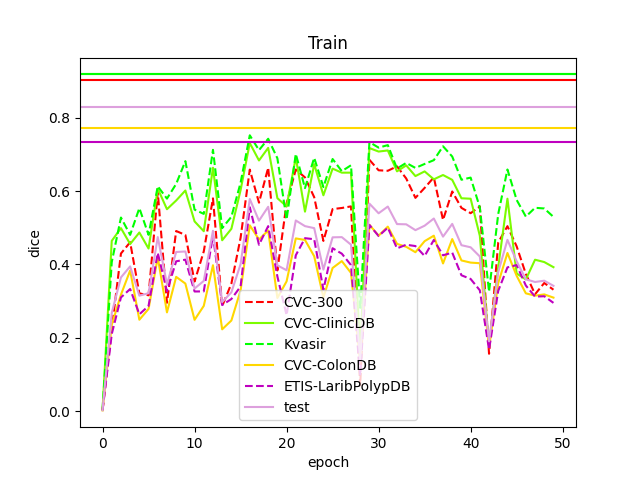
\includegraphics[width=\linewidth]{Figures/50-plot.png}
	\caption{The graph shows the trend of the value of Dice on all 6 types of images based on the current epoch. As we can see, the model obtains higher values with certain sets of images and lower ones with others.}
	\label{fig:fig1}
\end{figure}


\section{Conclusion}

In conclusion, this paper presents a comprehensive investigation into the problem of polyp segmentation in endoscopic imaging. Through the implementation of the hybrid semantic network (HSNet) combined with the RW loss function, we have addressed key challenges in the field, including semantic gaps, detail recovery, and global context modeling.

Our experimental results on multiple challenging polyp segmentation datasets, including Kvasir-SEG, ClinicDB, ColonDB, Endoscene, and ETIS, demonstrate the effectiveness of HSNet compared to existing state-of-the-art models. However we are aware that the results obtained have significant margins of improvement, due to the fact that we had limited hardware resources at our disposal, which prevented us from fully leveraging the model. 

The incorporation of both CNN and Transformer components in HSNet allows for the separate capture of local and long-term features, leading to improved segmentation accuracy, while the utilization of the RW loss function further contributes to the optimization stability of the model and enhances its convergence during training.

Moreover, the introduction of the cross-semantic attention module (CSA) and the dual-branch hybrid semantic complementary module (HSC) in HSNet addresses the challenges of semantic gaps and detail restoration, resulting in more precise segmentation masks with restored appearance details.

Our study not only contributes to the advancement of polyp segmentation techniques but also sheds light on the potential benefits of hybrid models combining CNN and Transformer architectures in medical image analysis tasks. Finally, the proposed HSNet framework can serve as a foundation for future research and can be extended to other medical imaging applications beyond polyp segmentation.

\begin{figure}
    \centering
    \subfigure{
\includegraphics[width=0.15\textwidth]{Figures/148.png}}
    \subfigure{
\includegraphics[width=0.15\textwidth]{Figures/148-t.png}} 
    \subfigure{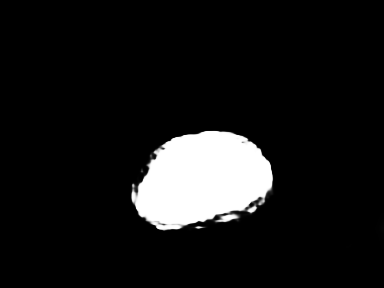
\includegraphics[width=0.15\textwidth]{Figures/148-p.png}}
    \caption{From left to right, in order: input image, true mask, predicted mask.}
    \label{fig:foobar1}
\end{figure}
\begin{figure}
    \centering
    \subfigure{
\includegraphics[width=0.15\textwidth]{Figures/165.png}}
    \subfigure{
\includegraphics[width=0.15\textwidth]{Figures/165-t.png}} 
    \subfigure{
\includegraphics[width=0.15\textwidth]{Figures/165-p.png}}
    \caption{From left to right, in order: input image, true mask, predicted mask.}
    \label{fig:foobar2}
\end{figure}



%----------------------------------------------------------------------------------------
%	 REFERENCES
%----------------------------------------------------------------------------------------

\printbibliography % Output the bibliography

%----------------------------------------------------------------------------------------

\end{document}
